

\documentclass{scrartcl}

\usepackage{graphicx,
            amsmath,
            subfigure,
            amsfonts,
		sidecap,
            tikz,
            bm,
		verbatim}
\usepackage{natbib}
\usepackage{graphicx}
\usepackage{algorithm}
\usepackage{algpseudocode}
\graphicspath{ {images/} }
\usepackage{amssymb}
\usepackage{amsthm}


\usepackage[pdftex]{hyperref}

\hypersetup{
colorlinks,%
citecolor=black,%
filecolor=black,%
linkcolor=black,%
urlcolor=black
}

\usetikzlibrary{arrows,positioning} 

\tikzset{
    select/.style={
           draw=black,
           line width=1.2mm
    },
    punkt/.style={
           circle,
           draw=black,
           minimum height=4em,
           text centered}
}

\renewcommand\arraystretch{1.2}
\newcommand{\f}[1]{\textbf{#1}}

\title{Gaussian Process Preference Learning for Creating Board Game Heuristics}

\subtitle{Lab Report: Development and Application Data Mining and Learning Systems - Winter Semester 2014/2015}

\date{05/03/2015}

\author{Vignesh Rao Yelluri \\ RWTH Aachen University \\ \texttt{yelluri.vr@gmail.com}}

\begin{document}

\maketitle


\begin{abstract}
We implement the active preference learning algorithm for learning the model of a  board game using Gaussian Processes. We consider Othello and Checkers board games which simulates a game for a pair of game heuristics and returns the preference or winner heuristic. These set of preferences are used to learn the game model. We have recast the preference learning into GP binary classification and then we can apply classical inference approaches like Expected Propagation to compute the posterior distribution. Since we are doing Active learning, our constraint is to learn with informative data and at a faster rate. This is done using the concept of Bayesian Active Learning by Disagreement (BALD) which tells what are the next best heuristics  to simulate a game and learn the model efficiently. Our ultimate goal is to predict the winners, given pairs of heuristics and create a best heuristic which has the best winning rate.
\end{abstract}

\section{Introduction}
	In this section, we briefly describe the board game heuristics and the basic idea of preference learning with these game heuristics.

\subsection{Board Game Heuristic}
	In order to play a game efficiently, a player needs the full min-max tree which helps us to find the next best move so that the player can try to win. But, construction of a full min-max tree itself is not easy. For example. the full min-max tree of Chess game has a total of $2.1\times10^{96}$ possible nodes which cannot be computed or stored. This motivates us to learn a heuristic without complete knowledge about the game. We have the min-max tree of limited depth for board games like Othello and Checkers. So a playing agent chooses its next best move based on a scoring function or heuristic which ranks the next possible moves at the leaves of the limited min-max tree. Here we also assume that the scoring function is a linear function of the board features. Precisely a heuristic is of the functional form $f(x) = W^{T}X_T$ , where $X$ is the game state at time $T$ and our is goal is to learn this weight vector $W$.

\subsection{Preference Learning}
	Preference learning is a task of making inference on the data which consists of a pair of items with a corresponding binary target class or label \cite{chu2005preference}. This label is the preferred item for a given pair of items. These kind of data exists in many real life scenarios like recommendation systems, decision making, graphics design etc. For Example. A person might prefer Audi over BMW, or given a news about FIFA one might prefer to give the label sports rather than politics.
 
\subsection{Gaussian Process Preference Learning}
	In our learning approach, we assume that there is latent or hidden utility function $f$ such that $f(\mathbf{h})$ is the value of the utility / strength of a game heuristic $\mathbf{h}$. For Example. $f(\mathbf{h}_i) > f(\mathbf{h}_j)$ simply means that heuristic $i$ is preferred / won over heuristic $j$. Bayesian methods is being used to learn this latent function $f$. This is done by modelling $f$ from a Gaussian Process Prior. Then we can compute the likelihood function and posterior distribution with which we can predict the preference / winner of a test pair of heuristics. The preference learning can then be recast as a special case of GP binary classification problem (see section 3.3). Probit likelihood used in Gaussian Process Classification is not a Gaussian and hence we cannot compute the posterior mathematically.  Hence approximations like Expected Propagation is used to infer the model.

\subsection{Active Learning Strategy}
	The process of simulating games is quite time consuming and we need large amount of training set of preferences to learn the model. Gaussian Process though efficient is very slow on learning with large data. This necessitates the need for learning with minimal training set of preferences. Training set which shall be generated on the fly also means that learning time must be as minimum as possible instead of taking some days to learn. Thus Active Learning Strategy implemented here makes the framework very much useful and efficient. The strategy called the Bayesian Active Learning by Disagreement (BALD)\cite{houlsby2012collaborative}, overcomes the previous challenges by finding the heuristic in the parameter space which the model is more uncertain about. This makes us to learn more significant parameter spaces in our model. Hence learning will be accelerated as we explore and learn new spaces which the model is uncertain about.


\section{Related Work}

Our work is based on [Houlsby, 2012], which introduces the new preference kernel which takes a pair of data points as input and translates the preference learning as GP binary classification. It also formulates the Bayesian Active Learning by Disagreement (BALD) objective function thus enabling to learn the model more efficiently. We investigated this concept of BALD objective and tried to find a new heuristic which has the best win rate / utility value and also learn efficiently. We fixed one heuristic in a heuristic pair and optimized the other heuristic by the optimization of BALD Objective. We have used the concept of Approximation from [Rasmussen, 2006], this book gives the basics of GP for machine Learning along with state of the art approximation techniques like Laplace Approximation and Expectation Propagation.

 \hfill \

Preference learning from discrete choice data [Eric, 2008] has discussed about active learning strategy for learning iteratively and efficiently. It also explains sequence of steps in finding a best data point with highest valuation on inferring directly the latent function $f$. Our work is inspired by the sequence of steps from this paper to learn efficiently. Our method is also based on [Chu, 2005], which presents preference learning using Gaussian processes . From this paper, the concept of probit likelihood and model selection by optimizing the hyperparameters using gradient based algorithm are used in the pyGPs framework which we use in our project. The pyGPs framework \cite{NeuMarHuaKer15} provides most of the functionalities for machine learning using Gaussian Processes, on top of which we added the preference kernel and mean functions.


	
	\section {Approach}
We implement this learning tool in python platform. We use a game simulator for Othello and Checkers to simulate games and return the winner which can be augmented to the training data set. For Gaussian Process Preference Learning, we use the pyGPs framework from python from which we can use off the shelf functionalities like posterior and prediction. We then implemented the new preference mean and co-variance function which can be contributed to the pyGPs \cite{NeuMarHuaKer15} framework. This learning tool is assumed to perform well for board games where the heuristic is a linear function of the board features.

\subsection {Active Preference Learning}
The main goal of active learning is to achieve higher accuracy and faster rate of learning using fewer training examples. In other words, we have to learn the game model as quickly as possible \cite{eric2008active}. By doing this, we ensure the data in our training set to be more valuable i.e. of higher information gain avoiding less important, random, repetitive data. Thus we choose Gaussian Processes which is powerful in learning accurately combined with BALD objective which makes learning even faster with fewer examples \cite{houlsby2012collaborative}.


\newpage
To learn efficiently we follow these sequence of steps:

\begin{algorithm}
\caption{Steps for Active Preference Learning}
\begin{algorithmic}
\State Generate $k$ random heuristics 
\State Simulate games among these heuristics
\State Record the results in training dataset
\For {$N$ rounds}
\State Find the top scoring heuristic from the training set
\State For this fixed top scorer, find an opponent by optimizing the BALD Objective (14)
\State Benchmark this opponent to calculate its strength
\State Append this opponent to the training set
\State Simulate games with this new heuristic and update the training dataset
\State Infer the Model by Expectation Propagation
\State Calculate the accuracy by prediction on test cases.

\EndFor	
\end{algorithmic}

\end{algorithm}




		
\subsection{Preference Learning Model}

	We assume a latent utility function f exists, which tells us the strength of a game heuristic. We try to learn this latent preference function $f:\mathcal{X}\mapsto \mathbb{R}$ which we consider as a Gaussian Process. A Gaussian Process is completely defined by the mean and co-variance function. We define this mean and co-variance function of $f(x)$ as 

	\begin{equation}
m(x) = \mathbb{E} [f(x)],
\end{equation}


\begin{equation}
k(x,x\prime) = \mathbb{E}[(f(x) - m(x))(f(x\prime)-m(x\prime))]
\end{equation}

and now the Gaussian Process is represented as

\begin{equation}
f(x) \sim \mathcal{GP} (m(x),k(x,x\prime)) 
\end{equation}


	We place a GP prior on function $f$, i.e. before seeing any data, we have a prior belief that the mean function would be 0 and RBF kernel can be a good co-variance function. The Radial Basis Function(RBF) kernel can be expressed as,

\begin{equation}
k(x , x\prime) = \sigma_f^2 \exp( - \frac {1}{2l^2}(x - x\prime)^2)
\end{equation}


where, parameters $\sigma_f^2$ is the signal variance and $l$ is the length scale. So given a pair of heuristics $\mathbf{h}_i,\mathbf{h}_j\in\mathcal{X}$. We simulate the game and record the result. We assumed that the utility function can tell us which heuristic is strong given a pair, we represent the result as $f(\mathbf{h}_i) > f(\mathbf{h}_j)$ if heuristic $\mathbf{h}_i$ has won over heuristic $\mathbf{h}_j$, and $f(\mathbf{h}_j) > f(\mathbf{h}_i)$ if $\mathbf{h}_j$ has won. The target variable $y\in\{-1,1\}$ can be set to $y=+1$ if the first heuristic in a given heuristic pair has won and $y=-1$ otherwise. When a game ends in a draw, we try to record 2 preference results with $y=+1$ and $y=-1$ so the uncertainty is not lost. We can now compute the likelihood function\cite{chu2005preference} of  $f$ given $\mathbf{h}_i$, $\mathbf{h}_j$ and $y$

	\hfill 
	
	\vspace{-0.65cm}
{\small
\begin{align}
\mathcal{P}(y|\mathbf{h}_i,\mathbf{h}_j,f) &= \Phi[(f[\mathbf{h}_i] - f[\mathbf{h}_j])y]\,,\label{eq:likelihood}
\end{align}
}

\vspace{-0.7cm}

\hfill

\normalsize 
where $\Phi(z) = \frac{1}{\sqrt{2\pi}} \int_{-\infty}^{z}\exp( -t^2/2) dt$ is the standard Gaussian cumulative distribution function.
	


\subsection {Recast the Preference Model}
	It is evident that the likelihood of function $f$ is just the difference $f(\mathbf{h}_i)$ - $f(\mathbf{h}_j)$ and we can capture this difference into another function $g:\mathcal{X}^2\mapsto\mathbb{R}$ which is also a Gaussian process $g(\mathbf{h}_i,\mathbf{h}_j) = f(\mathbf{h}_i) - f(\mathbf{h}_j)$. This has the new preference mean and preference co-variance function from mean $\mu$ and co-variance $k$ of function $f$ as follows
	
\begin{equation}
\mu_\text{pref}(g_\text{ij}) = \mu(f_i) - \mu(f_j)
\end{equation}


\begin{equation}
k_\text{pref}((\mathbf{h}_i,\mathbf{h}_j),(\mathbf{h}_k,\mathbf{h}_l)) = k(\mathbf{h}_i,\mathbf{h}_k) + k(\mathbf{h}_j,\mathbf{h}_l) - k(\mathbf{h}_i,\mathbf{h}_l) - k(\mathbf{h}_j,\mathbf{h}_k)
\end{equation}

	

Note that function $g(h_i,h_j)$ takes 2 heuristics as input, and hence it's mean and co-variance functions also takes 2 heuristics as inputs. Since  $g$ is defined from $f$ through a linear operation, a GP prior on $f$ induces a GP prior on $g$. We can learn the function $g$ ignoring $f$ since it will be learnt implicitly by definition.
Also we are learning the difference in function $g$ which means we are interested more in the sign of the value instead of the exact magnitude of the difference during prediction of the winner. 

\hfill \\

 The likelihood of function $g$ is defined as 

\hfill 

	\vspace{-0.65cm}
{\small
{\small
\begin{align}
\mathcal{P}(y|\mathbf{h}_i,\mathbf{h}_j,g) &= \Phi[g(\mathbf{h}_i, \mathbf{h}_j)y]\,.\label{eq:likelihood2}
\end{align}
}

\vspace{-0.7cm}

\hfill 
\normalsize

The Combination of this likelihood with a GP prior based on preference kernel translates the pairwise preference learning problem into GP binary classification \cite{houlsby2012collaborative}. The GP prior defines any function with the given prior mean and co-variance function. The likelihood function conditions the prior function to be consistent with the observed training data. Thus choosing the functions which are consistent with data and rejecting others gives us the posterior distribution. The posterior distribution is nothing but the combination of GP prior and likelihood function (8).

\newpage

\subsection {Inference by approximating Posterior and Predictions}
 The usage of probit likelihood for GP classification is not a Gaussian and hence it cannot be analytically tractable. Thus we can use inference approximation techniques like Expectation Propagation \cite{rasmussen2006gaussian}. In this state of the art algorithm, we compute local likelihood functions which form the marginal cavity distribution. Then we compute the Gaussian approximation to this marginal. We try to minimize the KL divergence between the actual posterior and the approximation such that we can compute a good estimate of the posterior and later can predict the winner of the game, given a heuristic pair. The approximate posterior is given as


\begin{equation}
q(g|X,y) \triangleq \frac {1}{Z_\text{EP}}p(g|X) \prod_{i=1}^{n}t_i(g_i|\widetilde{Z_i},\widetilde{\mu_i},\widetilde{\sigma_i}^{2}) = \mathcal{N}(\mu,\Sigma),
\end{equation}

where $\mu$ and $\Sigma$ are,


\begin{equation}
\mu = \Sigma\widetilde{\Sigma}^{-1}\widetilde{\mu} \quad , \quad \Sigma = (K^{-1} + \widetilde{\Sigma}^{-1})^{-1}
\end{equation}

here $q(g|X,y)$ is the approximation of the posterior $p(g|X,y)$, $Z_\text{EP}$ is the approximated marginal likelihood and $p(g|X)$ is the GP prior of $g$. The tilde parameters $\widetilde{\mu} , \widetilde{\Sigma}$ and $\widetilde{Z}$ are for the local likelihood approximations, where $\widetilde{\mu}$ is the vector of $\mu_i$ and $\Sigma_i$ is the diagonal with $ \widetilde{\Sigma}_\text{ii} = \widetilde{\sigma_i}^{2}$. The local likelihood approximation of mean and variance at each site $i$ is calculated by



\begin{equation}
\widetilde{\mu_i} = \widetilde{\sigma_i}^{2}(\widehat{\sigma_i}^{-2}\widehat{\mu_i} - \sigma_\text{-i}^{-2}\mu_\text{-i})
 \quad , \quad 
\widetilde{\sigma_i}^{2} = ( \widehat{\sigma_i}^{-2} - \widetilde{\sigma}_\text{-i}^{-2} )^{-1}
\end{equation}


here $\widehat{\mu_i}$ and $\widehat{\sigma_i}^{2}$ are the marginal moments which is derived by assuming that the first and second moments are equal since we minimize $KL(p(g|X,y)||q(g|X,y))$ divergence between the actual and approximate posterior. The parameters $\mu_\text{-i}$ and $\sigma_\text{-i}^{2}$ are the cavity distribution which includes all cases except for site $i$. Also the marginal posterior variance $ \widehat{\sigma_i}^{2}$ is always larger than the cavity variance $ \sigma_\text{-i}^{2}$ and hence site variance $\sigma_i^{2} > 0$ \cite{rasmussen2006gaussian} is always true.


\hfill 

In the case of Predictions, the test point or pair of heuristics as in our case is denoted as $x_* = [h_\text{1*},h_\text{2*}]$. According to Gaussian Process, the test and training points are jointly Gaussian. Hence the predicted mean and variance of test pair is given by

\begin{equation}
\mathbb{E}_q[g_*|X,y,x_*] = k_*^{T}(K + \widetilde{\Sigma})^{-1}\widetilde{\mu}
 \quad, \quad
\mathbb{V}_q[g_*|X,y,x_*] = k(x_*,x_*) -  k_*^{T}(K + \widetilde{\Sigma})^{-1} k_*
\end{equation}

here $k(x_*,x_*)$ is test by test variance and $K$ is the train by train variance. $k_*$ is nothing but the train by test variance since the test and train points are jointly Gaussian. (Note: we use the same preference kernel which takes in pairs of heuristics). Having the mean and variance of the function value $g$ at $x_*$, we can compute the probability that heuristic 1 has won the game from the formula given below,



\begin{equation}
q(y_*=+1|X,y,x_*) = \Phi(\dfrac{k_*^{T}(K + \widetilde{\Sigma})^{-1}\widetilde{\mu}}{\sqrt{1+  k(x_*,x_*) -  k_*^{T}(K + \widetilde{\Sigma})^{-1} k_*}})
\end{equation}


This formula calculates the cumulative standard normal distribution $\Phi$ and hence the value is strictly in the range (0,1) since it gives us the probability of win for heuristic 1 $(y=+1)$. In order to predict who is the winner given a pair of heuristic, we can define that, if the probability is greater than 0.5, heuristic 1 has won or heuristic 2 otherwise. Also we can squash this function to the range (-1,+1) using a squash function. Then if the value is positive, we predict heuristic 1 has won or heuristic 2 otherwise.

Another important factor for the efficiency of the learning are the values of parameters used in co-variance kernel (4) like $l,\sigma_f$ and likelihood function. We optimize these hyper parameters $\theta =( l,\sigma_f)$ by any gradient based optimization algorithm by maximizing the log marginal likelihood \cite{chu2005preference}. The prediction can now be efficient enough for the given dataset.



\subsection {Optimizing the BALD Objective}
In Active Learning we are supposed to learn the function $g$ with minimal training dataset. Thus we need to identify a new pair / tuple of game heuristics $x = [ h_i , h_j]$ where $h_i$ and $h_j$ are 2 different heuristics, which has the maximum information gain. In other words, the new heuristic pair maximizes the expected reduction in posterior entropy. Now that we are able to compute the predictive mean and variance for any pair of heuristics, we can easily obtain the mean $\mu_x$ and variance $\sigma_x^2$ of a heuristic pair. The BALD algorithm \cite{houlsby2012collaborative} chooses a heuristic pair $x$ which maximizes the objective

\hfill 

\vspace{-0.5cm}
{\small
\begin{equation}
\mathrm{h} \left[ \Phi\left( \mu_x(\sigma_x^2 + 1)^{-1/2} \right)\right] -
C(\sigma_x^2 + C^2)^{-1/2} \exp\left(-\mu_x^2(2\left(\sigma_x^2+ C^2\right))^{-1}\right)\,.\label{eqn:BALD}
\end{equation}
}

\vspace{-0.6cm}

\hfill 

\normalsize
where $\mathrm{h}[g]=- g\log g - (1-g)\log(1-g)$ is the binary entropy function and constant term $C=\sqrt{\pi\log 2 / 2}$. The Objective has a maximum value when the model is uncertain about the winner ($\mu_x$ almost 0), and has high uncertainty about the function value($\sigma_x^2$ is large). The second term prevents the objective function to sample in regions where the model knows that the outcome is uncertain. This optimization can be done with a bfgs optimizer in python. This learns the parameter space where there is high uncertainty, rather than just learning an uninformative parameter space. We then simulate a game for this new heuristic pair and update the dataset. 

 Having defined the BALD objective, we propose to use this for finding the best heuristic having a high win rate. We choose a top scoring heuristic from the current training sample, for this top scorer we try to optimize an opponent heuristic by maximizing BALD objective. The BALD chooses the heuristic which is as powerful as the top scorer heuristic and also highly uncertain about the outcome. As we learn iteratively, the parameter space with high uncertainty is learnt and eventually we come up with the best heuristic. We have done experiments on this in next section.

\newpage

\section{Experiments}

We have conducted experiments with Othello and Checkers Board game. We have applied the above techniques to prove the correctness and efficiency of our method. The initial parameters of this experiment are, having 2 initial opponents, each game is played 3 times to avoid noise, and the depth of the min-max tree used is 4. The function $f$ has zero mean as prior mean function and RBF kernel as the prior co-variance function. We then set prior mean and co-variance of function $g$ from equation (5) and (6) by having the mean and co-variance of function $f$ as input. We used the standard probit likelihood since this is Gaussian process Classification and since this likelihood is not a Gaussian, we used the Expectation Propagation Approximation for inferring the posterior mean and variance of the model. At each iteration, we also optimized the hyper parameters $\mathrm{\theta}$ by Gradient descent algorithm of pyGPs \cite{NeuMarHuaKer15}.


\subsection {Accuracy Plots}

\begin{figure}[H]

      \includegraphics[width=0.5\textwidth]{othello/accuracy}
\includegraphics[width=0.5\textwidth]{checkers/accuracy}
  \caption{Plot for Accuracy Vs No. of Runs for the game Othello (left) and Checkers (right). The algorithm runs for 100 iterations and at each iteration we measure the accuracy by predicting the winners given 1000 test heuristic pairs. Initially we started with 2 heuristics in the training set and found a new heuristic pair at each iteration and simulated games.}
\end{figure}



At each iteration, we used the BALD objective to find 1 entirely new heuristic pair without fixing any one of the heuristic in the pair. For prediction, the model outputs the mean and variance of function $g(h_1,h_2)$ given 2 heuristics $h_1$ and $h_2$ where the sign of mean value tells us which heuristic has won that particular game. If the mean value is negative, the second heuristic in the pair is predicted to win or the first heuristic is predicted to win if the mean value is non-negative. The accuracy for the game Othello is 45\% at the start and gradually rises to 82\% at iteration 65 and then saturates. Similarly, the accuracy of game Checkers is 47\% at the start and gradually rises to 84\% at iteration 83 and then saturates. This shows the BALD objective function is efficient in learning the model with good accuracy estimates and as early as possible, since the total runtime for each of this experiment is approximately 45 minutes.


\subsection {Benchmarking Best Heuristic}

\begin{figure}[H]

      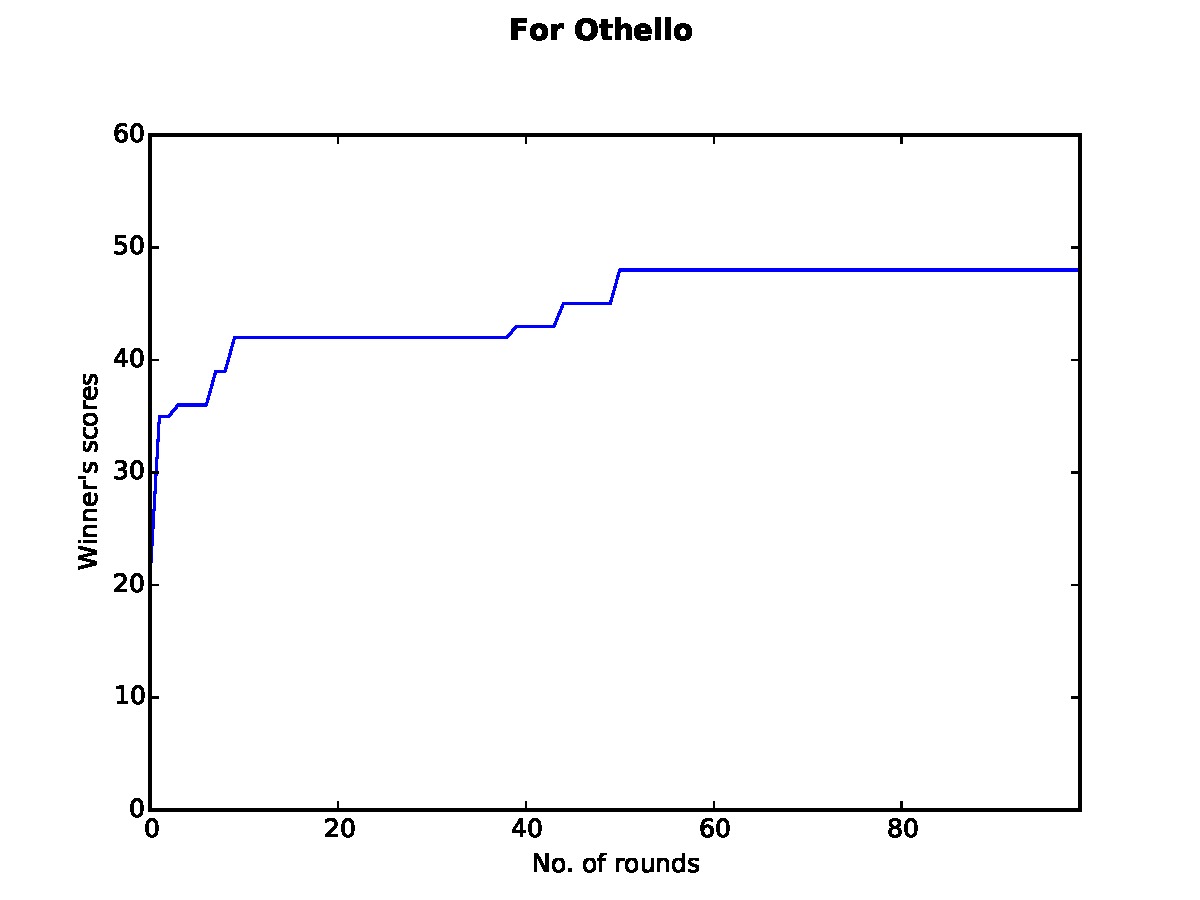
\includegraphics[width=0.5\textwidth]{othello/realwins}
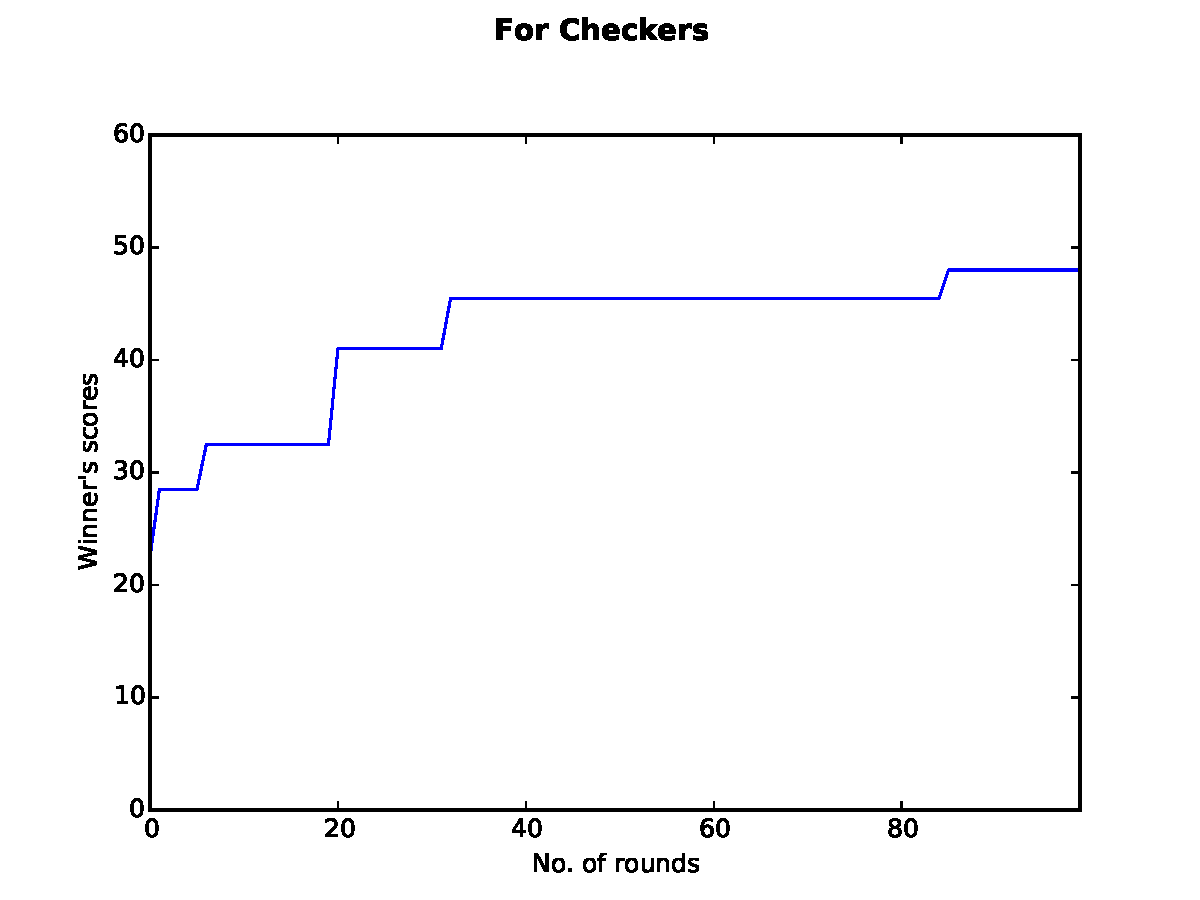
\includegraphics[width=0.5\textwidth]{checkers/realwins}
  \caption{Plot for the Score of the best heuristic Vs No. of Runs for the game Othello (left) and Checkers (right). At each round, we tried to find an opponent for the top scoring heuristic in the current training set. And then we calculated the benchmark score / winning rate of the best heuristic found so far by us, which can either be in training set or newly found opponent. For details, see the description below.}
\end{figure}

The above experiment has 100 rounds / iterations in total. This experiment is different from the one in section (4.1) since, it doesn't find an entirely new heuristic pair / tuple, instead it fixes the first heuristic as the top scorer heuristic and optimizes the other heuristic by BALD Objective. We experiment whether this might help us in finding the best heuristic. Also the accuracy of this model has no change on doing the BALD optimization by this way. In this experiment initially we had 5 random heuristics, simulated games among them and inferred the model. Now at each iteration, we found the top scoring heuristic in training set. This is done by benchmarking / playing games against 50 randomly generated heuristics and calculating the score of a heuristic as the cumulative sum of 1 if it wins, 0.5 if its ends in a draw or 0 if it has lost with each of the opponent in the 50 random benchmark heuristics. Thus the maximum score a heuristic can achieve is 50, when it has won all games over these benchmark opponents. Now for this top scoring heuristic in the current training set, we find its opponent by optimizing the BALD objective. This is done by fixing first heuristic in the heuristic pair as current top scoring heuristic and trying to find the second heuristic in that pair by optimizing the BALD. By doing this, we find an opponent to be as strong as the top scoring heuristic. Then, we append this opponent to the training set after simulating games with some 5 randomly selected heuristics from the training set and learn the model. Now at each iteration, we plotted the benchmark score of the best heuristic found so far as the heuristic which has top score in either the training set or newly found heuristic by optimizing the BALD. The score of the best heuristic found is 47 and 48 at  $57^{th}$ and $82^{nd}$ iteration for Othello and Checkers board game respectively. Note that the score of the best heuristic is strictly increasing because, we consider the newly found opponent as the best heuristic only if it has higher benchmark score than the previous best heuristic. Otherwise, the previous best heuristic remains to be the best heuristic so far. 



\subsection {Mean and Variance plots}

\begin{figure}[H]

      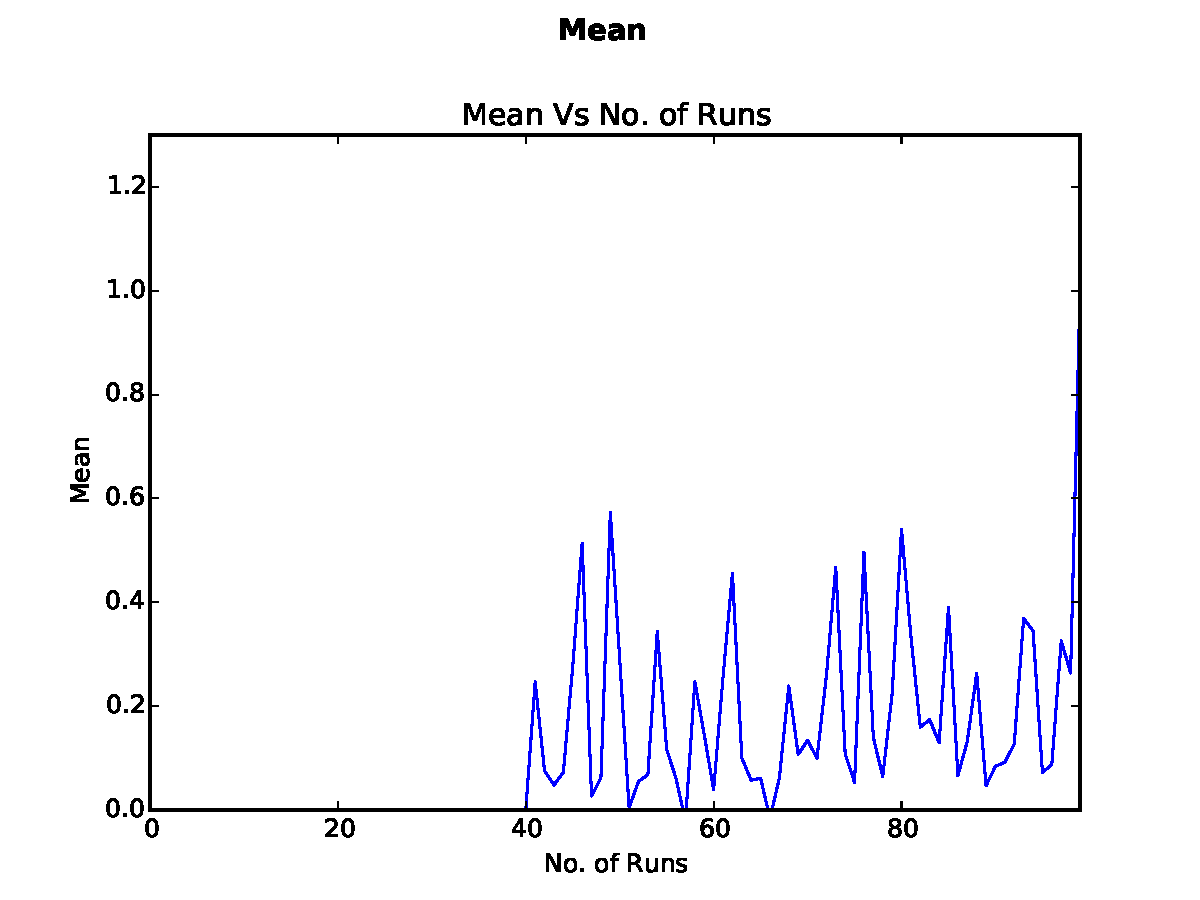
\includegraphics[width=0.5\textwidth]{othello/Mean}
\includegraphics[width=0.5\textwidth]{othello/variance}
  \caption{Plot of Mean (left) and Variance (right) Vs No. of Runs for the game Othello. These plots are for the same experiment in section (4.2) for Othello, and plotted the mean and variance of the heuristic pair found by optimizing only the second heuristic in this pair.}
\end{figure}

It is interesting to see how the Bayesian Active Learning by Disagreement (BALD) Objective function (14) optimizes a new heuristic pair such that, it chooses a heuristic pair whose strength(mean) between 2 heuristics are almost same and highly uncertain(variance) about the outcome of the game. Note that the mean of function $g(h_1,h_2)$ tells us about the outcome of the game. It's magnitude tells the relative strength of the winner heuristic and sign tells which heuristic in this pair is the winner. The variance of function $g(h_1,h_2)$ is nothing but the certainty / confidence about the winner. Its value is close to 0 when one of the heuristic is relatively much stronger, and high variance means uncertainty about which heuristic is the winner. The BALD Objective is used to learn the parameter space with highest uncertainty. As we learn iteratively, the parameter space is explored better and better making the variance/uncertainty to reduce. Due to reduction in uncertainty, the relative strength(mean) between the 2 heuristics increases. Both these trends are consistent with the plots above.

\newpage


\section{Conclusions}

We have implemented the Active Preference Learning algorithm to learn the board game model for Othello and Checkers using Gaussian Processes, and also able to find the best board game heuristic having high win rate. We have done preference learning as a special case of Gaussian Process Binary classification by using the preference kernel. We have investigated and tested that, implementing the BALD Objective by fixing the first heuristic in the pair to be top scorer heuristic and optimizing the opponent of the top scoring heuristic would enable us to learn efficiently and also can find the best heuristic having high win rate. This method has also been verified by the experimental results for its correctness.





\bibliography{bib/reference}{}
\bibliographystyle{plain}

\end{document}



